\chapter{Modulação deleuzeana, modulação algorítmica e manipulação midiática}

\begin{flushright}
\emph{João Francisco Cassino}
\end{flushright}

Qual é a diferença entre os conceitos de \emph{manipulação} e de
\emph{modulação}? Este texto tem por objetivo propor uma visão de que os
dois termos, apesar de muito próximos, são diferentes e não devem ser
utilizados para definir as mesmas coisas. Mais do que isso, sugere
diferenciar \emph{modulação} em duas partes: a clássica \emph{modulação
deleuzeana} e a \emph{modulação algorítmica}. Como forma de exemplificar
esta proposição serão utilizados casos das mídias tradicional,
eletrônica e digital e também do \emph{marketing} corporativo. Como
contexto histórico, mostrar"-se"-á a transição da \emph{sociedade
disciplinar}, nascida nos séculos \versal{XVIII} e \versal{XIX}, para a \emph{sociedade de
controle}, típica do final do século \versal{XX} e deste início do século \versal{XXI},
que surge com as tecnologias de comunicação em massa e, mais
recentemente, com o advento e popularização das tecnologias digitais em
rede. O gráfico 1 mostra o fluxo de pensamento a ser desenvolvido nesta
abordagem .

\begin{figure}[!ht]
%\begin{minipage}{0,4\textwidth}
\centering
  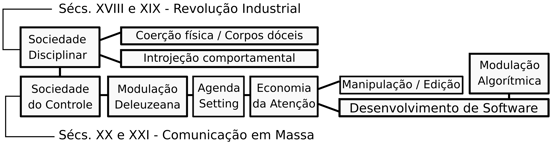
\includegraphics[width=80mm]{./imgs/grafico1.png}
\caption{GRÁFICO 1 -- Fluxo de Desenvolvimento Teórico}
%\end{minipage}
 \end{figure}

\section{Sociedade Disciplinar e Sociedade do Controle}

Decorrente do pensamento de Michel Foucault (1989), a \emph{sociedade
disciplinar} se caracteriza quando, com a função de \emph{docilizar
comportamentos,} o poder passa a ser aplicado sobre os corpos dos
indivíduos, inclusive pela \emph{coerção física}. A instrumentalização
das disciplinas precisa da existência de instituições disciplinares,
todas criadas, da forma mais ou menos como as conhecemos hoje, em meados
do século \versal{XVIII}, para suprir as necessidades que surgem com a Revolução
Industrial, com o êxodo do rural para o urbano e com a aparição do
operário fabril. São dessa mesma época as escolas, os hospitais, as
casas de loucos (manicômios) e a prisão pan"-óptica de Jeremy Benthan --
instituições que teriam por função docilizar e vigiar as pessoas
adequando"-as às necessidades do novo modelo capitalista emergente. Aqui
há sempre uma autoridade presente, que ensina, comanda e diz o que
fazer: o professor, o médico, o psiquiatra, o carcereiro. As
instituições feitas para disciplinar os seres humanos têm por derradeiro
objetivo \emph{introjetar o comportamento} dentro de cada pessoa,
criando hábitos, impondo uma cultura que, mesmo na ausência da
vigilância da autoridade, garanta que o agir e o pensar sigam as normas
previamente ditadas.

Já a \emph{sociedade de controle}, como explica Lazzarato:

\begin{quote}
exerce seu poder graças às tecnologias de ação a distância da imagem, do
som e das informações, que funcionam como máquinas de modular e
cristalizar as ondas, as vibrações eletromagnéticas (rádio, televisão),
ou máquinas de modular e cristalizar pacotes de bits (...) (2006, 85)
\end{quote}

A \emph{modulação}, portanto, tem por poder modular, cristalizar, uma
determinada subjetividade desejada na memória, no cérebro das pessoas.

\begin{quote}
Se as disciplinas moldavam os corpos ao constituir hábitos,
principalmente na memória corporal, as sociedades de controle modulam os
cérebros, constituindo hábitos sobretudo na memória mental
(Lazzarato,2006,86).
\end{quote}

Em síntese, a \emph{sociedade disciplinar} precisa da ação da autoridade
sobre os corpos, até mesmo da punição física, para a introjeção
comportamental. Já a \emph{sociedade de controle} é mais sutil, ocorre à
distância, penetrando os cérebros e forjando as mentes com seus
mecanismos de influência. Portando, o conceito de \emph{modulação},
criado pelo filósofo francês Gilles Deleuze e amplamente utilizado pelo
sociólogo Maurizio Lazzarato, é a base da \emph{sociedade de controle}.

Manuel Castells (2017, p. 209) explica como funcionam os mecanismos de
enquadramento da mente. Para ele, o processamento de informações que
relacionam o conteúdo e o formato da mensagem com molduras
(\emph{frames}) são ativados por mensagens geradas na esfera da
comunicação. O poder de quem gera essas informações, no entanto, é
limitado por como as pessoas selecionam e interpretam essas informações.
Citando a pesquisa \emph{Pew Global Attitudes Project}, Castells
ressalta que somente cerca de 7\% das matérias publicadas na mídia nos
Estados Unidos da América despertaram muita atenção dos telespectadores,
a maioria delas é relativa à segurança ou às violações de normas
sociais. \emph{``O ódio, a ansiedade, o medo e o grande entusiasmo são
particularmente estimulantes e também são retidos na memória de longo
prazo''} (Castells, 2017, p. 209), escreve. Quando mecanismos emocionais
são estimulados, o cérebro ativa a capacidade de decisão de nível
superior, buscando e dando mais atenção às informações que recebe. É por
isso que o enquadramento (\emph{framing}) é baseado na provocação de
emoções (ibid, p. 210). Como consequência, o jornalismo abusa do
sensacionalismo e o \emph{marketing} procura atingir os sentimentos dos
consumidores. Inclua"-se na lista de Castells o elemento da erotização,
fortemente presente nos conteúdos midiáticos.

\section{Agenda Setting e Economia da Atenção}

Para o enquadramento de mentes, uma das formas mais poderosas de
influência da mídia sobre seus consumidores é a técnica chamada de
Agenda \emph{Setting}. Como explica o professor Clóvis de Barros Filho
(1996, p. 28), o termo refere"-se à hipótese na qual a agenda temática
dos meios de comunicação impõe os temas de discussão social. Se a mídia
tradicional veicula matérias sobre a Copa do Mundo de Futebol, por
exemplo, espera"-se que a sociedade, nos escritórios, nas salas de aulas
e nos bares, debatam também sobre a Copa do Mundo. Se o agendamento
temático é a violência do tráfico de drogas, esta vira a pauta dos
corredores, dos cafezinhos e nos trens. Clóvis de Barros lembra o
\emph{slogan} de uma extinta emissora de \versal{TV}: \emph{``Aconteceu Virou
Manchete''}. Logo, presume"-se que se não virou manchete, não aconteceu.
A mesma lógica pode se aplicar ao \emph{slogan} \emph{``Globo e você,
tudo a ver''}. Há aqui um duplo sentindo: pode significar conexão total
com o telespectador, mas também que tudo o que há para se ver, para se
assistir, está na Globo (pelo menos o que há de relevante).

\begin{quote}
\emph{Esta construção da realidade social operada pelos meios, por
intermédio de uma seleção e uma hierarquização arbitrária de eventos,
produz efeitos: promove discussões sociais encapsuladas pela barreira do
desconhecimento dos temas jogados no lixo das reuniões de pauta dos
jornais, ou dos que nem chegaram a ela}, escreve (Barros, 1996, p. 28).
\end{quote}

Os editores escolhem quais assuntos serão revelados ao público e quais
serão completamente e deliberadamente ignorados, geralmente sob a
desculpa de falta de tempo (na \versal{TV} e no rádio) ou de falta de espaço em
páginas impressas (em jornais e revistas). Mas os temas que são de
interesse comercial ou político das emissoras ganham horas e horas e
horas dedicadas na programação.

A \emph{modulação} deleuzeana, base da \emph{sociedade de controle}, que
disputa os espaços nos cérebros das pessoas, usando para tal técnicas de
enquadramento emocional (\emph{framing}) e de imposição de temas na
agenda de debates da vida cotidiana da sociedade (\emph{Agenda Setting})
é tanto um recurso de poder político, social e ideológico quanto um
modelo de negócios altamente lucrativo que sustenta o enorme
conglomerado de mídia mundial.

Em 1971, Herbert A. Simon afirmou que em um mundo repleto de
informações, surge um novo tipo de escassez: a atenção do consumidor.
``Portanto, uma grande quantidade de informações cria uma pobreza de
atenção e uma necessidade de alocar essa atenção eficientemente entre a
superabundância de fontes de informação que poderiam consumi"-la'',
escreve no texto \emph{Designing Organizations for an Information"-rich
World} (p. 40-41). Tal pensamento estimularia que vários pensadores,
tais como Thomas H. Davenport e John C. Beck, passassem a utilizar o
termo ``Economia da Atenção'' para propagar como as organizações
empresariais podem se beneficiar do que eles chamam de uma ``nova moeda
para os negócios''. Entendem que os mercados hoje são ``motores movidos
pelo combustível da atenção''. A atenção é atualmente para as empresas o
que as fazendas e os campos foram para as sociedades rurais, o que as
fábricas foram para a Revolução Industrial e o que o conhecimento é para
a Era da Informação.

\begin{quote}
\emph{Mas agora, como os fluxos de informações desnecessárias entopem os
cérebros dos trabalhadores e das comunicações corporativas, a atenção é
um recurso raro que verdadeiramente dá poder a uma empresa} (\versal{DAVENPORT};
\versal{BECK}, 2001, p. 17).
\end{quote}

Dizem ainda que a atenção é um recurso valioso que precisa ser
gerenciado como qualquer outro recurso precioso. Uma prova são as
pesquisas chamadas \emph{Top of Mind}, realizadas anualmente, que no
\emph{marketing} empresarial são usadas para qualificar quais são as
marcas mais populares nas mentes dos consumidores. Por meio de
entrevistas, pergunta"-se qual é o nome do primeiro sabão em pó que lhe
vem à cabeça, do primeiro refrigerante, do primeiro tênis, da primeira
marca de produtos eletrônicos e assim por diante. Com isso, mede"-se a
eficiência e a eficácia de uma campanha de publicidade. As marcas mais
lembradas, mais cristalizadas nos cérebros, são as vencedoras desta
competição empresarial. No Brasil, a pesquisa é realizada anualmente
pelo Instituto DataFolha e resulta no prêmio Folha Top of Mind. Em 2017,
as marcas campeãs foram, pela ordem, Omo (com 7\% de menções), Coca"-Cola
(4\%), Nike (4\%) e Samsung (4\%).

Por definição, a gestão de \emph{marketing} tem por um de seus
objetivos:

\begin{quote}
criar ou identificar valor, produzindo inovações estratégicas em
produtos, processos e modelagem de negócios, a partir de um profundo
conhecimento do perfil e das demandas dos mais diferentes públicos e
mercados (\versal{LIMA}, M.; et al., 2007, p. 19, apud. Branstad e Lucier, 2001).
\end{quote}

Essa descrição vai ao encontro do que destaca Lazzarato (2006, p. 101),
de que o \emph{Marketing} tem como uma de suas funções ser capaz de
\emph{criar mundos} como uma das forças de agenciamento de expressão.
Mais do que isso, o \emph{marketing} seria o centro estratégico das
empresas, pois a prática mercadológica seria a de reduzir as
possibilidades das criações e das escolhas, com foco em forçar as opções
sob o jugo de decisões pré"-definidas pelas corporações. Tais opções são
limitadas, mas se mostram como liberdade de escolha aos compradores, mas
a liberdade de escolher se resume ao que as empresas ofertam.

\begin{quote}
As sociedades de controle caracterizam"-se assim pela multiplicação da
oferta de `mundos' (de consumo, de informação, de trabalho, de lazer).
Trata"-se porém de mundos lisos, banais, formatados, porque são mundos da
maioria, vazios de toda singularidade'', escreve (\versal{LAZZARATO}, p. 2006,
101).
\end{quote}

Mas, pergunta Lazzarato (2006, p. 103), como o \emph{marketing} pode
produzir a mudança na sensibilidade do consumidor e estimulá"-lo a
comprar? Que tipo de subjetivação é mobilizada pela publicidade? Para
ele, o turbilhão de encadeamento de imagens e sons cria uma nova
sensibilidade em quem assiste àquele conteúdo. Revela um mundo possível
que existe, mesmo que exista somente no universo da própria propaganda.
Referem"-se aos signos de mundos possíveis, gerando desejos de
pertencimento a esses mundos (assim como frustrações por não conseguir
integrá"-los). Justamente ao criar mundos e propagá"-los -- e impedir que
outras multiplicidades concorrentes se constituam -- é quando a
\emph{sociedade de controle} assume a forma da expropriação capitalista
contemporânea (2006, p. 178).

Criar mundos custa caro. O investimento em \emph{marketing} é tão
importante quanto o desenvolvimento e a fabricação dos próprios produtos
e consome parte considerável da verba das empresas. A pesquisa \emph{\versal{CMO}
Spend Survey 2017-2018} da consultoria Gartner, que anualmente questiona
os principais executivos de \emph{marketing} (\emph{Chief Marketing
Officers}) sobre o quanto e como gastam seus recursos, mostrou que entre
os anos 2014 e 2017, os investimentos no setor estiveram em torno de
11,3\% a 12,1\%, em média, para cerca de 350 grandes empresas
respondentes. Note que se trata de corporações com faturamento
bilionário. Dez porcento de \versal{US}\$ 1 bilhão são \versal{US}\$ 100 milhões,
verdadeiras fortunas. Porém, dependendo do setor, como o do cinema
norte"-americano, o investimento em divulgação pode ser equivalente a
50\% do quanto se gastou para produzir o filme. Um fato a observar aqui
é a tendência de investimento das empresas -- dois terços dos \versal{CMO}s
disseram que planejam aumentar a verba de propaganda digital, enquanto
as mídias tradicionais deverão perder recursos progressivamente.

O livro \emph{A Estratégia do Oceano Azul -- Como Criar Novos Mercados e
Tornar a Concorrência Irrelevante}, de W. Chan Kim e Renée Mauborgne, é
um \emph{best seller} bastante recomendado por professores de cursos de
\versal{MBA} em Gestão Empresarial ou de Gestão de \emph{Marketing}. A premissa é
simples: o oceano da competição do mercado é um oceano vermelho,
manchado de sangue pela concorrência brutal (metaforicamente falando),
repleto de rivais que lutam entre si por uma parcela de lucros cada vez
menor. O segredo do oceano azul é gerar novos e intocados espaços de
mercado prontos para o crescimento. ``Os oceanos azuis se definem como
espaços de mercado não aproveitados e pela criação de demanda e
oportunidades para um crescimento altamente rentável'', escrevem (2005,
p. 5). Nos oceanos azuis, a competição perde sua validade e as regras
daquele jogo ainda não existem. Assim, \emph{oceano azul} pode ser
comparada com a \emph{criação de mundos} descrita por Lazzarato. A
criação de oceanos azuis deve ser contínua. Há cem anos, indústrias como
a automobilística, a de aviação ou a petroquímica simplesmente não
existiam. Da mesma forma, um estudo da consultoria McKinsey, de 2017,
afirma que, até o ano de 2030, entre 400 e 800 milhões de profissionais
vão perder seus empregos. De 800 profissões, em 46 países, até um terço
dos trabalhos atuais poderão ser automatizados em pouco mais de uma
década.

\section{Modulação deleuzeana, Modulação Algorítmica e Manipulação}

Se a \emph{modulação deleuzeana} é ocupar espaço nos cérebros à
distância, utilizando técnicas de enquadramento mental, de agendamento
temático e de retenção da atenção para \emph{criar mundos} e vender
\emph{oceanos azuis}, em seu interior está indubitavelmente contida a
ação de \emph{manipular} conteúdos de mídia, sejam tradicionais,
eletrônicos ou digitais. No entanto, a \emph{modulação deleuzeana} é
mais ampla do que a mera \emph{manipulação}. O gráfico 2 propõe uma
estrutura de conjuntos de quatro itens que compõem a \emph{modulação
deleuzeana:}



\begin{figure}[!ht]
%\begin{minipage}{0,4\textwidth}
\centering
  \includegraphics[width=60mm]{./imgs/grafico2.png}
\caption{GRÁFICO 2 -- Subconjuntos da Modulação Deleuzeana}
%\end{minipage}
 \end{figure}

O primeiro subconjunto, o jornalismo informativo, tem por função básica
a prestação de serviço à comunidade e dar informações relevantes àquele
povo, cidade ou país. Quando, por exemplo, cai uma ponte que obstrui a
principal avenida de uma localidade, o jornalismo, até para se
viabilizar como produto de mídia e ter credibilidade para disputar a
Economia da Atenção, precisa noticiar aquele fato. Nem sempre o editor
vai querer manipular a realidade, pelo contrário, dependendo da
situação, pode pôr em prática o ideal da reportagem imparcial, que apura
informações e consulta várias fontes.

O segundo item, a propaganda e o \emph{marketing} não esconde do
consumidor que sua intenção é vender"-lhe produtos, portanto, por mais
que utilize técnicas de sedução do cliente, não há que se falar em
``manipulação'', pois o desejo de influenciar é explícito.

Por \emph{manipulação}, entendemos, em língua portuguesa\footnote{Fonte:
  Dicionário Online Priberam -
  \emph{www.priberam.pt/dlpo}}, o
ato de preparar com as mãos, manusear, manejar, condicionar, influenciar
-- geralmente em proveito próprio, adulterar, falsificar. A
\emph{manipulação de mídia} é uma técnica bastante utilizada tanto no
meio tradicional quanto nos meios digitais. Surge, porém, com a mídia
\emph{broadcast} (que consiste em enviar, projetar e transmitir um mesmo
conteúdo em larga escala, atingindo o maior número de pessoas possível).
O caminho do \emph{broadcast} é de mão única: parte de um emissor e
atinge um receptor. Há diversas teorias de comunicação que estudam
profundamente o problema -- da Escola de Frankfurt a Jesús
Martín"-Barbero, com interpretações profundamente diferentes. A relação
emissor"-receptor, portanto, guarda similaridade com as \emph{sociedades
disciplinares} e suas figuras de autoridade professor"-aluno,
médico"-paciente, psiquiatra"-louco, carcereiro"-prisioneiro. Temos aqui as
relações \versal{TV}"-telespectador, rádio"-ouvinte, jornal"-leitor. A mídia
limitada pelo \emph{broadcast} precisa lançar mão de estratégias e
táticas diversas para atingir seus objetivos de modulação. A
\emph{manipulação} é uma delas. Um exemplo notório do que é manipular
(preparar com as mãos) foi a edição do último debate presidencial das
eleições brasileiras de 1989, a primeira pós"-redemocratização, ocorrido
em 14 de dezembro, entre Fernando Collor de Mello e Luiz Inácio Lula da
Silva. O caso é estudado em praticamente todas as faculdades de
jornalismo, um episódio quase obrigatório. No dia seguinte ao debate, a
Rede Globo de Televisão veiculou duas matérias, uma no Jornal Hoje e
outra no Jornal Nacional, ambas desequilibradas, mas foi a segunda que
gerou grande polêmica. A emissora selecionou os melhores momentos do
candidato que apoiava (Collor) e os momentos com pior desempenho de Lula
. Além disso, foi destinado a Collor um minuto e meio a mais do que ao
candidato petista. No final da década de 1980, quando não existia o
contraponto das redes sociais digitais, a força do principal programa
jornalístico da Globo tinha um poder de influência muito maior do que é
hoje (e que ainda é muito forte). Naquele dia, o \versal{JN} atingiu 66 pontos na
pesquisa Ibope, que mede a audiência televisiva. Conforme publicado no
\emph{site} \emph{http://memoriaglobo.globo.com}, a própria emissora admite que:

\begin{quote}
``(...) os responsáveis pela edição do Jornal Nacional afirmaram, tempos
depois, que usaram o mesmo critério de edição de uma partida de futebol,
na qual são selecionados os melhores momentos de cada time. Segundo
eles, o objetivo era que ficasse claro que Collor tinha sido o vencedor
do debate, pois Lula realmente havia se saído mal(Memorial Rede Globo,
online)
\end{quote}

Desta forma, nota"-se que a manipulação se deu porque alguém, um editor,
assistiu ao debate, minuto a minuto, capturou trechos de seu interesse,
montou uma ordem como um quebra"-cabeça, com seus próprios dedos,
literalmente, com o objetivo de induzir o voto de quem assistia. Esse é
o ponto central na proposição que é feita neste capítulo: a manipulação
-- ressalte"-se -- precisa ter intenção de ludibriar a interação humana,
mesmo que fazendo uso de recursos tecnológicos de comunicação. É preciso
realizar a ação de manejar, de pôr em prática, de colocar
deliberadamente em funcionamento uma dinâmica que induza, que iluda.

O quarto subconjunto, a \emph{modulação algorítmica}, pode sim ter o
objetivo de influenciar comportamentos como a \emph{manipulação de
mídia}, mas funciona de forma completamente diversa. Lazzarato diz que o
\emph{marketing} via Internet toca os indivíduos em sua singularidade e
os reduz a mostras nos bancos de dados, diferenciando os consumidores em
nichos específicos de forma muito mais eficiente do que se faz com meras
pesquisas de mercado (2006, p. 182).

A mecânica é simples: ao depender do conteúdo veiculado pelas emissoras
televisivas (\emph{broadcast}), o espectador fica restrito à pauta
estabelecida pelos veículos de comunicação (agenda \emph{setting}). Na
rede mundial de computadores, o conteúdo é buscado conforme o interesse
direto e imediato do internauta. Por exemplo, na época em que as músicas
eram ouvidas somente via rádio ou pela emissora \versal{MTV}, os fãs de uma banda
ou de um músico mantinham seus aparelhos ligados e esperavam muito tempo
para escutar uma determinada canção. Contavam com a boa vontade (e com o
interesse comercial) de quem fazia a programação musical. Hoje, com os
serviços de \emph{streaming}, como YouTube e Spotify, a música é
desfrutada no momento que se quer. O consumo de conteúdo é sob demanda.
Com esta nova realidade de \emph{modulação algorítmica}, \emph{manipular
a mídia} torna"-se uma técnica muito restrita para exercer a
\emph{modulação deleuzeana}.

A Inteligência Artificial, operada por \emph{softwares}, é a ``alma''
dos robôs e dos dispositivos autômatos. Grandes e diversificadas bases
de dados são os insumos que os algoritmos de inteligência artificial
precisam para trabalhar. Quanto mais informações disponíveis às
máquinas, mais condições elas terão de apresentar um melhor desempenho
analítico e preditivo aos seus utilizadores. Já \emph{Big Data} é o nome
dado pelo mercado para o armazenamento, integração, processamento e
tratamento destas gigantescas bases de dados geradas cotidianamente pela
sociedade global conectada. Como explica o professor de direito
norte"-americano Frank Pasquale, em seu livro \emph{The Black Box
Society} (2015), o \emph{Big Data} permite o funcionamento de um
complexo padrão de técnicas de reconhecimento e análise de massivos
volumes de dados que buscam racionalizar decisões e substituir
intermediários. De posse da enorme quantidade de dados pessoais
recolhidas pela inteligência artificial e processadas por \emph{Big
Data}, os profissionais de marketing e os desenvolvedores de softwares
têm um colosso de oportunidades jamais visto para criar mundos e vender
oceanos azuis, ampliando os lucros de suas empresas.

O sociólogo Sérgio Amadeu da Silveira, em seu livro \emph{Tudo Sobre Tod@s -- Redes Digitais, Privacidade e Venda
de Dados Pessoais}, explica que o processamento e mineração de
informações envolve a agregação dos dados coletados e armazenados pelas
tecnologias digitais, enriquecendo o perfil pessoal de cada indivíduo de
maneira bastante detalhada (2017, eBook Kindle, posição 889). Estes
perfis e coletas criam enormes oportunidades para novos produtos e
serviços\emph{. Como escreve Hayash:}

\begin{quote}
(...)\versal{LIMA}, M.; et al., 2007, p. 23), ``as atividades do processo de
gestão de marketing dependem necessariamente de algum tipo de
conhecimento de mercado. Um mundo em mudança exige constante coleta de
informações para assegurar a capacidade de atender às demandas dos
mercados (\ldots{}) (2001. In: \versal{LIMA}, M.; et al., 2007, p. 23).
\end{quote}

Philip Kotler e Kevin L. Keller, no livro \emph{Administração de
Marketing}, escrevem que:

\begin{quote}
``telefones celulares, video"-games e a Internet estão reduzindo a
atenção dada à mídia tradicional, bem como a interação social face a
face uma vez que as pessoas ouvem música ou assistem a um filme em seus
telefones celulares. Os profissionais de marketing devem acompanhar as
seguintes tendências tecnológicas (2013, p. 85).
\end{quote}

Os canais de comunicação de \emph{marketing} digital, como
\emph{websites}, e"-mails, blogs, plataformas de áudio e vídeos digitais
são importantes ferramentas de ponto de contato e de encontro na rede
mundial de computadores e fornecem \emph{feedback} aos seus
administradores. Esta é a principal diferença para o mundo do
\emph{broadcast}. Nas mídias digitais, os canais são bidirecionais ou
multidirecionais. Da mesma forma que a \emph{sociedade de controle} não
substituiu a \emph{sociedade disciplinar}, mas a complementou, as redes
digitais interativas não substituíram as redes de \emph{broadcast}, mas
as influenciaram e as complementaram. Serviços de Internet, como os
grandes portais Universo Online (\versal{UOL}) ou G1 (Globo.com), são ferramentas
\emph{online} que tentam reproduzir a lógica do agenda \emph{setting} e
do \emph{broadcast}. O fato é que a \emph{modulação} precisa ser feita
agora mais do que pela mera \emph{manipulação} midiática, de um editor
humano, mas pela mediação de algoritmos, de inteligência artificial,
subsidiados por gigantescas bases de dados, cujos resultados de
influência na retenção da atenção e nas decisões de compra são sim
pré"-definidas por profissionais humanos de \emph{marketing} e
desenvolvedores de \emph{softwares}, mas que as sugestões de indução de
consumo são efetuadas por máquinas que tentam prever os comportamentos
dos consumidores fundamentadas por experiências anteriores. Kotler e
Keller (2013, p. 73) descrevem o caso da empresa \emph{Best Buy}, que
montou uma base de dados de 15 terabytes de 75 milhões de residências.
Foram captadas todas as formas de interação com clientes (telefonemas,
cliques de \emph{mouse}, cupons de desconto). Algoritmos classificaram
100 milhões de clientes em categorias (fanáticos por tecnologia, mãe
moderna, profissional bem"-sucedido, pai de família). Com essas
informações, a empresa emprega \emph{marketing} de precisão para
\emph{modular} clientes e melhorar suas vendas. O consumidor capturado,
ranqueado e categorizado por um \emph{novo mundo}, por um \emph{oceano
azul}, tem reforçada sua posição de refém dos dispositivos de poder
capitalista para produção e apropriação de riquezas.

\section{Conclusão}

A evolução da \emph{sociedade disciplinar}, dos séculos \versal{XVIII} e \versal{XIX}, que
dependia da presença física da autoridade e muitas vezes do castigo
corporal para garantir a docilidade das pessoas em favor do sistema
dominante, soma"-se nos séculos \versal{XX} e \versal{XXI} às técnicas da \emph{sociedade
de controle}, que permite modular cérebros à distância. O conceito de
modulação, proposto por Gilles Deleuze e trabalhado por Lazzarato, pode
ser decomposto em subconjuntos, dentre os quais os mais relevantes para
este capítulo são a \emph{manipulação midiática} e a \emph{modulação
algorítmica}. Enquanto a manipulação exige que um ser humano exerça o
manejo de uma ação planejada para direcionar um conteúdo de mídia
\emph{broadcast}, a modulação algorítmica usa as mais avançadas técnicas
de inteligência artificial para induzir os comportamentos dos usuários
das tecnologias de informação e comunicação. Por ter acesso a uma enorme
quantidade de dados pessoais de cada indivíduo e gerida por códigos
computacionais, a modulação algorítmica atua de maneira personalizada,
prevendo gostos e preferências de cada um, sendo a tecnologia mais
eficaz para \emph{criar mundos}, gerar \emph{oceanos azuis} e vender
produtos ou ideias.

\section{Referências}

\versal{BARROS FILHO}, Clóvis de. \textbf{Agenda setting e educação.} In:
Comunicação e Educação -- Revista do Departamento de Comunicações e
Artes da \versal{ECA}/\versal{USP}. São Paulo, 1996, pp. 27 a 33. Disponível em:
\emph{www.revistas.usp.br/comueduc/article/view/36219}. Acesso em 7 de junho de 2018.

\versal{BASTA}, D.; \versal{MARCHESI}, F.R. de A.; \versal{OLIVEIRA}, J. A. F. De; Sá, L. C. S. de.
\textbf{Fundamentos de Marketing} -- 7ª Edição. Série Gestão
Empresarial. Rio de Janeiro. Editora \versal{FGV}, 2006.

\versal{CASTELLS}, Manuel. \textbf{O Poder da Comunicação}, pp. 209-210. 2ª
Edição. Rio de Janeiro / São Paulo. Editora Paz e Terra, 2017.

\versal{DAVENPORT}, Thomas H.; \versal{BECK}, John C. \textbf{The Attention Economy:
Understanding the New Currency of Business}, pp. 17. Harvard Business
Press, 2002

\textbf{Debate Collor x Lula.} In: Memória Globo. Online. Disponível em:
\emph{http://memoriaglobo.globo.com/erros/debate-collor-x-lula.htm}.
Acesso em 7 de junho de 2018.

\versal{FOUCAULT}, Michel . \textbf{Microfísica do poder.} 8ª. ed. Rio de
Janeiro: Graal, 1989.

\versal{GREGÓRIO}, Rafael. \textbf{Omo, Coca-Cola, Nike e Samsung são as marcas
mais lembradas no Brasil.} In: Folha de S.Paulo, 30 de outubro de 2017.
Disponível em:
\emph{www1.folha.uol.com.br/topofmind/2017/10/1930576-omo-coca-cola-nike-e-samsung-sao-as-marcas-mais-lembradas-no-brasil.shtml}.
Acesso em 7 de junho de 2018.

\versal{KIM}, Chan \& \versal{MAUBORGNE}, Renée. \textbf{A Estratégia do Oceano Azul --
como criar novos mercados e tornar a concorrência irrelevant}e; Rio de
Janeiro: Campus, 2005.

\versal{KOTLER}, P.; \versal{KELLER}, Kevin L. \textbf{Administração de marketing.} 14.
ed. São Paulo: Pearson Prentice Hall, 2013.

\versal{LAZZARATO}, Maurizio. \textbf{As revoluções do capitalismo.} Civilização
Brasileira, 2006.

\versal{LAZZARATO}, Maurizio. \textbf{Signos, máquinas e subjetividades.} São
Paulo: Edições \versal{SESC}-\versal{SP}: n-1 edições, 2014.

\versal{LIMA}, M.; \versal{SAPIRO}, A.; \versal{VILHENA}, J.B.; \versal{GANGANA}, M. \textbf{Gestão de
Marketing} -- 8ª edição revista e atualizada. Rio de Janeiro. Editora
\versal{FGV}, 2007.

\versal{MCINTYRE}, Ewan; Virzi, Anna Maria. \textbf{\versal{CMO} Spend Survey 2017-2018:
Budgets Recede Amid Demand For Results}. Gartner Inc. 2017.

\versal{PASQUALE}, Frank. \textbf{The black box society: The secret algorithms
that control money and information.} Harvard University Press, 2015.

\versal{SILVEIRA}, Sérgio Amadeu. \textbf{Tudo Sobre Tod@s: redes digitais,
privacidade e venda de dados pessoais.} São Paulo: Edicões \versal{SESC}, 2017,
online.

\versal{SIMON}, Herbert A. \textbf{Designing Organizations for an
Information-Rich World}, pp. 40-41. In M. Greenberger (Ed.), Computers,
communications, and the public interest. Baltimore, \versal{MD}: The Johns
Hopkins Press, 1971.
